% Define the rings. Store them in macros to make things
% more flexible. 
\def\ringa{(-1,0) circle (2) (-1,0) circle (3)}
\def\ringb{(1,0) circle (2) (1,0) circle (3)}

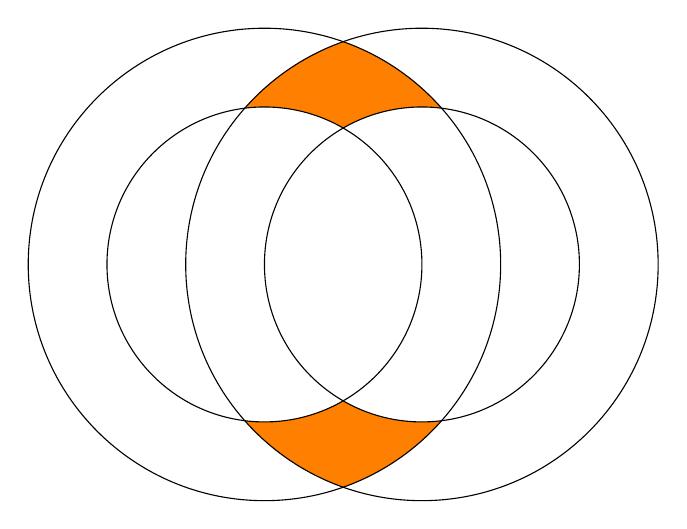
\begin{tikzpicture}
    % First we fill the intersecting area
    % The \clip command does not allow options, therefore 
    % we have to use a scope to set the even odd rule. 
    \begin{scope}[even odd rule]
        % Define a clipping path. All paths outside ringa will
        % be cut because the even odd rule is set. 
        \clip \ringa;
        % Fill ringb. Since the even odd rule is set, only the
        % ring will be filled, not the hole in the middle.  
        \fill[fill=orange] \ringb;
    \end{scope}
    % Then we draw the rings
    \draw \ringa;
    \draw \ringb;
\end{tikzpicture}